\chapter{Time Dependent Variational Principle}\label{make}

Das grundlegende Prinzip der Time-Dependent Variatonal Principle, kurz TDVP, ist die Äquivalenz der zeitabhängigen Schrödingergleichung
 zu einem Extremisierungspropblem einer Wirkungsfunktion $S=\int_{t_1}^{t_2}L \thinspace dt$ mit der Lagrange-Funktion:

\begin{align}
    L\left(\overline{\Psi}(t), \Psi(t), t\right)=\frac{i}{2}\langle\Psi(t) \mid \dot{\Psi}(t)\rangle-\frac{i}{2}\langle\dot{\Psi}(t) \mid \Psi(t)\rangle-\langle\Psi(t)|\hat{H}(t)| \Psi(t)\rangle
\end{align}

Eine explizite Herleitung der Äquivalenz ist in (...) zu finden. \\

\noindent Für die Verwendung des Variationsverfahren ist es notwendig, dass der zu variierende Ansatz-Wellenfunktion 
$\ket{\Psi(\mu_1,...,\mu_N}$ analytisch ist. Da die Normierungsfunktion $N=N(\mu,\muk)$ nicht analytisch ist, wird sie 
für den modifizierten Ansatz ausgelassen. Da ein normierter Ansatz in diesem semi-klassischen Minimierungsverfahren nicht 
von Notwendigkeit ist, lassen sich folgende Bewegungsgleichungen hinschreiben:
\begin{align}
    i\dot{\mu_i} &= \sum_{j}\left(G_{ij}\right)^{-1}\thinspace \partial_{\overline{\mu_j}}\mathcal{H}
\end{align}

mit 
\begin{align}
    G_{ij} &= \frac{\bra{\partial_{\overline{\mu_i}}\Psi}\ket{\partial_{\mu_j}\Psi}}{\N} 
    - \frac{\bra{\partial_{\overline{\mu_i}}\Psi}\ket{\Psi}\bra{\Psi}\ket{\partial_{\mu_j}\Psi}}{\N^2} \\
    \mathcal{H} &= \frac{\bra{\Psi}\hat{H}\ket{\Psi}}{\N}
\end{align}

\noindent mit der Konvention: $\bra{\partial_{\overline{\mu_j}}\Psi} = \left(\thinspace\ket{\partial_{\mu_j}\Psi}\thinspace\right)^\dagger$

\noindent Mit dieser modifizierten Gram-Matrix $G_{ij}$ und dem modifizierten Hamiltonian $\mathcal{H}$, ist die Normierung wieder 
gesichert. 

\newpage











\section{Wahl der Wellenfunktion}
\begin{wrapfigure}{r}{0.4\textwidth}
    \centering
    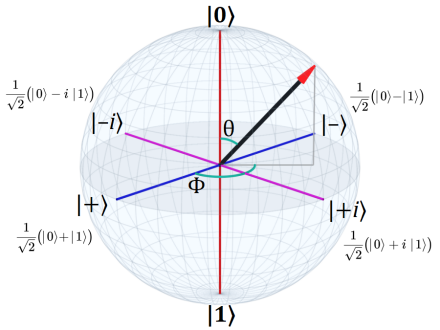
\includegraphics[width = 0.35\textwidth]{Abbildungen/bloch-sphere.png}
    \caption{Schematischer Aufbau einer Bloch-Sphere}
    \label{fig:qubit}
\end{wrapfigure}
Zur Vereinfachung werden alle Kernspin (wie der Elektronenspin) als 1/2-Spins angenähert. 
Die Wellenfunktion $\ket{\Psi}=\ket{\Psi(\mu_1(t),...,\mu_N(t)}$ enthält die zeitabhängigen Parameter $\mu_i(t)$ und realisiert einen 
kohärenten Zustand. Wir nutzen die Geometrie des 1/2-Spins aus und verwenden zur Darstellung die bekannte \textbf{Bloch-Sphäre}. 
Ähnlich wie die komplexe e-Funktion dank trigonemtrische Eigenschaften einen Kreis auf der Zahlenebene abbilden kann, ist es auch möglich,
 jeden Punkt auf einer Kugel zu beschreiben. Deshalb wählen wir folgenden Ansatz:

\begin{align}
    \ket{\Psi(\mu_1(t),...,\mu_N(t))} &= \prod_{i=1}^{N} \frac{1}{\sqrt{1+\mu_i\muk_i}}e^{\mu_i\thinspace S_i^-}\ket{\uparrow,...,\uparrow}
\end{align}

\section{ein 1/2-Spin im konstanten Magnetfeld}
Zum besseren Verständnis des TDVPs ist die beispielhafte Betrachtung des vereinfachten Falles sehr aufschlussreich. 
Zudem lassen sich Identitäten herleiten, die in die Erweiterung zum \textbf{Central Spin Model} Wiederverwendung finden werden.
Für den N=1 vereinfacht sich der Ansatz zu:
\begin{align*}
    \ket{\Psi} &= e^{\mu\thinspace S^-}\ket{\uparrow} \\
            &= (1 + \frac{\mu\thinspace S^{-}}{1!} + \frac{\left(\mu\thinspace S^{-}\right)^2}{2!} + ...)\ket{\uparrow}    \\
            &= \ket{\uparrow} + \mu\ket{\downarrow}
\end{align*}

\noindent Im folgenden haben wir uns die Eigenschaft des 1/2-Spins $\left(S^{-}\right)^{n}\ket{\uparrow}=0$  (n = 2,3,...) verwendet.

Der Hamiltonian lautet:
\begin{align}
    \hat{H} &= \gamma \vec{B}\hat{\vec{S}} = \gamma\left(B_x\hat{S}_x+B_y\hat{S}_y+B_z\hat{S}_z \right) \\
    &= \gamma \frac{B_x}{2}\Bigl(\ket{\downarrow}\!\bra{\uparrow}+\ket{\uparrow}\!\bra{\downarrow}\Bigr) \\
    & + \gamma \frac{iB_y}{2}\Bigl(\ket{\downarrow}\!\bra{\uparrow}-\ket{\uparrow}\!\bra{\downarrow}\Bigr) \\
    & + \gamma \frac{B_z}{2}\Bigl(\ket{\uparrow}\!\bra{\uparrow}-\ket{\downarrow}\!\bra{\downarrow}\Bigr) 
\end{align}

\noindent mit $\vec{B} = (B_x,B_y,B_z)^T$ und $\gamma=\mu_B\thinspace g_e$, wobei $\mu_B = 9.27 \cdot 10^{24} \frac{J}{T}$ das Bohrsche 
Elektronenmagneton und dem g-Faktor des freien Elektrones $g_e\approx 2$. Der Spin-Vektororperator 
$\hat{\vec{S}}= \frac{1}{2}\left(\hat{\sigma}_x,\hat{\sigma}_y,\hat{\sigma}_z\right)^T$ mit den Pauli-Matrizen $\hat{\sigma}_i$.\\ \\

und somit folgt für den \textbf{modifizierten Hamiltonian}:
\begin{align}
    \mathcal{H} &= \frac{\gamma}{2}\frac{B_x(\mu +\muk) + iB_y(\muk - \mu) + B_z(1-\mu\muk) }{1+\mu\muk}    \\
    \partial_{\muk} \mathcal{H} &= \frac{\gamma}{2} \frac{B_x(1-\mu^2) + iB_y(1+\mu^2) - 2\mu B_z}{(1+\mu\muk)^2} 
\end{align}

\noindent Im nächsten Schritt wird die von dem Haltionian unabhängigen \textbf{modifizierte Gram-Matrix $G_{ii}$} bestimmt, 
welche in diesem Fall eindimesnional ist.
Damit erhalten wir
\begin{align}
    G_{11} = \frac{1}{\left(1 + \mu\overline{\mu}\right)^2} \text{\space\space bzw.\space\space } G_{11}^{-1} = \left(1 + \mu\overline{\mu}\right)^2
\end{align}

\noindent Nach einer weiteren Rechnung ergibt sich auch der modifizierte Hamiltonian und dessen Ableitung:

\noindent Einsetzen in die DGL liefert:
\begin{align*}
    i\dot{\mu_i} &= \sum_{j}\left(G_{ij}\right)^{-1}\thinspace \partial_{\overline{\mu_j}}\mathcal{H} = \left(G_{ii}\right)^{-1}\partial_{\muk} \mathcal{H} \\
    &= \frac{\gamma}{2}B_x(1-\mu^2) + \frac{i\gamma}{2}B_y(1+\mu^2) -\mu \gamma B_z    \\
    \leftrightarrow \dot{\mu} &= \frac{1}{2}(B_y + iB_x)\mu^2 + \frac{1}{2}(B_y - iB_x) +i\mu \gamma B_z
\end{align*}

Die normierten \textbf{Spin-Erwartungswerte} $\frac{\bra{\Psi}\hat{\vec{S}}\ket{\Psi}}{\N}$ lauten:

\begin{align}
    \frac{\bra{\Psi}\hat{S_x}\ket{\Psi}}{\N} &= \frac{1}{2}\frac{\muk + \mu}{1+\mu\muk} = \frac{Re[\mu]}{1 + \mu\muk} \\
    \frac{\bra{\Psi}\hat{S_y}\ket{\Psi}}{\N} &= \frac{i}{2}\frac{\muk - \mu}{1+\mu\muk} = \frac{Im[\mu]}{1 + \mu\muk} \\
    \frac{\bra{\Psi}\hat{S_z}\ket{\Psi}}{\N} &= \frac{1}{2}\frac{1 - \mu\muk}{1 + \mu\muk}  
\end{align}
Bei dem Problem handelt es sich um die \textit{Larmor-Präzession}, indes die Lösung bereits bekannt ist. Zur Überprüfung reicht es,
 zu zeigen:
\begin{align}
    \frac{d}{dt}\left(\frac{\bra{\Psi}\hat{\vec{S}}\ket{\Psi}}{\N}\right) &= \gamma\vec{B} \cross \left(\frac{\bra{\Psi}\hat{\vec{S}}\ket{\Psi}}{\N}\right)
\end{align}


\begin{align}
    \partial_\mu \left(\frac{\bra{\Psi}\hat{S_x}\ket{\Psi}}{\N}\right)\dot{\mu} &= \frac{1}{2}\frac{1-\muk^2}{(1+\mu\muk)^2}\cdot\left[\frac{1}{2}(B_y + iB_x)\mu^2 + \frac{1}{2}(B_y - iB_x) +i\mu B_z\right]  \\
    \frac{d}{dt}\left(\frac{\bra{\Psi}\hat{S_x}\ket{\Psi}}{\N}\right) &= \partial_{\mu}\left[\frac{\bra{\Psi}\hat{S_x}\ket{\Psi}}{\N}\right]\dot{\mu} + \partial_{\muk}\left[\frac{\bra{\Psi}\hat{S_x}\ket{\Psi}}{\N}\right]\dot{\muk}\\
    &= B_y \frac{1}{2}\frac{1-\mu\muk}{(1+\mu\muk)^2} - B_z \frac{i}{2}\frac{\muk -\mu}{(1+\mu\muk)^2}    \\
    &= B_y\left(\frac{\bra{\Psi}\hat{S_z}\ket{\Psi}}{\N}\right) - B_z\left(\frac{\bra{\Psi}\hat{S_z}\ket{\Psi}}{\N}\right)
\end{align}
analog wird berechnet:
\begin{align}
    \frac{d}{dt}\left(\frac{\bra{\Psi}\hat{S_y}\ket{\Psi}}{\N}\right) &= B_z\left(\frac{\bra{\Psi}\hat{S_x}\ket{\Psi}}{\N}\right) - B_x\left(\frac{\bra{\Psi}\hat{S_z}\ket{\Psi}}{\N}\right)\\
    \frac{d}{dt}\left(\frac{\bra{\Psi}\hat{S_z}\ket{\Psi}}{\N}\right) &= B_x\left(\frac{\bra{\Psi}\hat{S_y}\ket{\Psi}}{\N}\right) - By\left(\frac{\bra{\Psi}\hat{S_x}\ket{\Psi}}{\N}\right)
\end{align}
Die Kreuzproduktstruktur lässt sich somit wiedererkennen.
